\documentclass[11pt,letterpaper]{article}

\addtolength{\oddsidemargin}{-.875in}
\addtolength{\evensidemargin}{-.875in}
\addtolength{\textwidth}{1.75in}

\addtolength{\topmargin}{-.875in}
\addtolength{\textheight}{1.75in}

\usepackage[utf8]{inputenc}
\usepackage{caption} % for table captions
\usepackage{amsmath} % for multi-line equations and piecewises
\DeclareMathOperator{\sign}{sign}
\usepackage{graphicx}
\usepackage{relsize}
\usepackage{xspace}
\usepackage{verbatim} % for block comments
\usepackage{subcaption} % for subfigures
\usepackage{enumitem} % for a) b) c) lists
\newcommand{\Cyclus}{\textsc{Cyclus}\xspace}%
\newcommand{\Cycamore}{\textsc{Cycamore}\xspace}%
\newcommand{\deploy}{\texttt{d3ploy}\xspace}%
\newcommand{\Deploy}{\texttt{D3ploy}\xspace}%
\usepackage{tabularx}
\usepackage{color}
\usepackage{multirow}
\usepackage{float} 
\usepackage[acronym,toc]{glossaries}
\newacronym{ANL}{ANL}{Argonne National Laboratory}
\newacronym{B4C}{B4C}{boron carbide}
\newacronym{BC}{BC}{boundary condition}
\newacronym{BOC}{BOC}{beginning of equilibrium cycle}
\newacronym{BSD}{BSD}{Berkeley Software Distribution}
\newacronym{BWR}{BWR}{Boiling Water Reactor}
\newacronym{CAISO}{CAISO}{California ISO}
\newacronym{CEA}{CEA}{Commissariat a l'Energie Atomique}
\newacronym{CFD}{CFD}{computational fluid dynamics}
\newacronym{CO2}{CO$_2$}{carbon dioxide}
\newacronym{CR}{CR}{control rod}
\newacronym{CRP}{CRP}{Coordinated Research Project}
\newacronym{CZP}{CZP}{Cold Zero Power}
\newacronym{DCC}{DCC}{depressurized conduction cool-down}
\newacronym{DOE}{DOE}{Department of Energy}
\newacronym[\glslongpluralkey={degrees of freedom}]{DoF}{DoF}{degree of freedom}
\newacronym{EOC}{EOEC}{end of equilibrium cycle}
\newacronym{FCEV}{FCEV}{Fuel Cell Electric Vehicle}
\newacronym{FDM}{FDM}{Finite Difference Method}
\newacronym{FEM}{FEM}{Finite Element Method}
\newacronym{FVM}{FVM}{Finite Volume Method}
\newacronym{FSV}{FSV}{Fort St. Vrain}
\newacronym[\glslongpluralkey={greenhouse gases}]{GHG}{GHG}{greenhouse gas}
\newacronym{GRS}{GRS}{Gesellschaft für Anlagen und Reaktorsicherheit}
\newacronym{H2}{H$_2$}{hydrogen}
\newacronym{He}{He}{helium}
\newacronym{HFP}{HFP}{Hot Full Power}
\newacronym{HPCC}{HPCC}{high pressure conduction cool-down}
\newacronym{HTE}{HTE}{High-Temperature Electrolysis}
\newacronym{HTGR}{HTGR}{High-Temperature Gas-Cooled Reactor}
\newacronym{HTR}{HTR}{High Temperature Reactor}
\newacronym{HTTR}{HTTR}{High Temperature Test Reactor}
\newacronym{HZDR}{HZDR}{Helmholtz-Zentrum Dresden-Rossendorf}
\newacronym{IAEA}{IAEA}{International Atomic Energy Agency}
\newacronym{icap}{iCAP}{Illinois Climate Action Plan}
\newacronym{INL}{INL}{Idaho National Laboratory}
\newacronym{IPyC}{IPyC}{inner pyrolytic carbon}
\newacronym{JFNK}{JFNK}{Jacobian-Free Newton-Krylov}
\newacronym{KAERI}{KAERI}{Korea Atomic Energy Research Institute}
\newacronym{Keff}{K$_{eff}$}{multiplication factor}
\newacronym{LBP}{LBP}{Lumped Burnable Poison}
\newacronym{LGPL}{LGPL}{Lesser GNU Public License}
\newacronym{LOCA}{LOCA}{loss of coolant accident}
\newacronym{LPCC}{LPCC}{low pressure conduction cool-down}
\newacronym{LTE}{LTE}{Low-Temperature Electrolysis}
\newacronym{LWR}{LWR}{Light Water Reactor}
\newacronym{MC}{MC}{Monte Carlo}
\newacronym{MHTGR}{MHTGR}{Modular High-Temperature Gas-Cooled Reactor}
\newacronym{MOC}{MOC}{middle of equilibrium cycle}
\newacronym{MOOSE}{MOOSE}{Multi-physics Object-Oriented Simulation Environment}
\newacronym{MPI}{MPI}{Message Passing Interface}
\newacronym{MSR}{MSR}{Molten Salt Reactor}
\newacronym{MTD}{MTD}{Champaign-Urbana Mass Transit District}
\newacronym{NEA}{NEA}{Nuclear Energy Agency}
\newacronym{NEM}{NEM}{Nodal Expansion Method}
\newacronym{NGNP}{NGNP}{Next Generation Nuclear Power}
\newacronym{NRC}{NRC}{Nuclear Regulatory Commission}
\newacronym{NSC}{NSC}{Nuclear Science Committee}
\newacronym{OECD}{OECD}{Organisation for Economic Co-operation and Development}
\newacronym{OPyC}{OPyC}{outer pyrolytic carbon}
\newacronym{ORNL}{ORNL}{Oak Ridge National Laboratory}
\newacronym{OS}{OS}{Operator-Splitting}
\newacronym{PBMR}{PBMR}{Pebble Bed Modular Reactor}
\newacronym{PDE}{PDE}{Partial Differential Equation}
\newacronym{PMR}{PMR}{Prismatic Modular Reactor}
\newacronym{PV}{PV}{photovoltaics}
\newacronym{RSC}{RSC}{Reserve Shutdown Control}
\newacronym{RSD}{RSD}{Relative Standard Deviation}
\newacronym{SD}{SD}{Standard Deviation}
\newacronym{SI}{SI}{Sulfur-Iodine}
\newacronym{SiC}{SiC}{silicon carbide}
\newacronym{SMR}{SMR}{Small Modular Reactor}
\newacronym{SNU}{SNU}{Seoul National University}
\newacronym{SOEC}{SOEC}{Solid Oxide Electrolysis Cells}
\newacronym{TIP}{TIP}{transverse integration procedure}
\newacronym{TRISO}{TRISO}{Tristructural Isotropic}
\newacronym{UIUC}{UIUC}{University of Illinois at Urbana-Champaign}
\newacronym{UNIST}{UNIST}{Ulsan National Institute of Science and Technology}
\newacronym{UK}{UK}{United Kingdom}
\newacronym{UMICH}{UMICH}{University of Michigan}
\newacronym{US}{US}{United States}
\newacronym{VHTR}{VHTR}{Very High Temperature Gas Cooled Reactor}
%\newacronym{<++>}{<++>}{<++>}
%\newacronym{<++>}{<++>}{<++>}

\definecolor{bg}{rgb}{0.95,0.95,0.95}
\newcolumntype{b}{X}
\newcolumntype{f}{>{\hsize=.15\hsize}X}
\newcolumntype{s}{>{\hsize=.5\hsize}X}
\newcolumntype{m}{>{\hsize=.75\hsize}X}
\newcolumntype{r}{>{\hsize=1.1\hsize}X}
\usepackage{titling}
\usepackage[hang,flushmargin]{footmisc}
\renewcommand*\footnoterule{}
\usepackage{tikz}

\usetikzlibrary{shapes.geometric,arrows}
\tikzstyle{process} = [rectangle, rounded corners, 
minimum width=1cm, minimum height=1cm,text centered, draw=black, 
fill=blue!30]
\tikzstyle{arrow} = [thick,->,>=stealth]

\graphicspath{}

\begin{document}

% --------- INTRO
% \section{Introduction}

\section{\glspl{PMR}}

% History
The history of prismatic \glspl{HTGR} or simply \glspl{PMR} begins in the 1960s with the deployment of the Dragon reactor in the \gls{UK}.
Its initial objective was to demonstrate the feasibility of the \gls{HTGR} and to launch the development of the technology.
The Dragon eeactor experiment first operated in July 1965 and reached full power of 20 MW$_t$ in April 1966.
The reactor operated for long periods at full power, demonstrated the successful operation of many components, and provided information on fuel and material irradiation tests.
Simultaneously, interest in the \gls{US} led to the 40 MW$_e$ \gls{HTGR} at Peach Bottom.
The reactor achieved initial criticality on March 1966 and went into commercial operation in June 1967.
Peach Bottom provided a valuable demonstration of the \gls{HTGR} concept by confirming the core physics calculations, verifying the design analysis methods, and providing a data base for further design activities.
Most importantly, the plant demonstrated the ability of \glspl{HTGR} to function in a load-following manner \cite{brey_development_2001}.
After the deployment of these two prototype reactors came the first \gls{HTGR} demonstration plant, the \gls{FSV} Generating Station.
Its electric power generation started in December 1976, reaching full-power operation in November 1981.
The \gls{FSV} plant generated 842 MW$_t$ to achieve a net output of 330 MW$_e$.
This reactor laid the foundation for future \gls{PMR} designs.
Beginning with \gls{FSV}, the \gls{US} core design included ceramic coated \gls{TRISO} particles embedded within rods placed in large hexagonal shaped graphite elements \cite{brey_development_2001}.
% Despite these plants did not demonstrate the commercial capabilities of the \glspl{PMR}, they were  valuable in demonstrating attributes as the performance of the \gls{TRISO} fuel particles \cite{herranz_power_2009}.

% Safety characteristics of HTGRs
The most fundamental characteristic of the \gls{PMR} is the unique safety philosophy embodied in its design \cite{iaea_current_2001}.
The control of radionuclides does not rely on active systems or operator actions.
\gls{TRISO} particles, Figure \ref{fig:triso}, play a big role in this task.
They consist of various layers acting in concert to provide a containment structure that limits radioactive product release.
A \gls{TRISO} particle is a microsphere of about 0.8 mm diameter.
It includes a fuel kernel surrounded by a porous carbon layer (or buffer), followed successively by an \gls{IPyC} layer, a \gls{SiC} layer, and an \gls{OPyC} layer.
An additional advantage of the \gls{TRISO} particles is that they increase the proliferation resistance of \glspl{HTGR}.
They are a very unattractive and the least desirable route for diversion or theft of weapons-usable materials \cite{huning_steady_2014}.
% The buffer layer allows for limited kernel migration and provides some retention of gas compounds \cite{oecd_nea_benchmark_2017}.
% The \gls{IPyC} layer protects the kernel from chloride during the \gls{SiC} decomposition and contributes to fission gas retention \cite{demkowickz_paul_triso_2019}.
% The \gls{SiC} layer ensures the structural integrity of the particle under constant pressure and helps retain non-gaseous fission products.
% The \gls{OPyC} layer contributes to fission gas retention and protects the \gls{SiC} layer during handling.

\begin{figure}[htbp!]
	\centering
	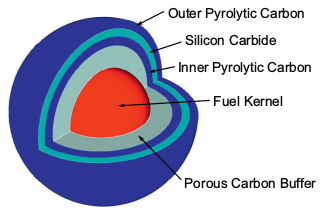
\includegraphics[height=3.5cm]{figures/triso}
	\caption{Drawing of a TRISO fuel particle. Image reproduced from \cite{hales_multidimensional_2013}.}
	\label{fig:triso}
\end{figure}

Another contributor to the passive safety of the \gls{HTGR} design is its materials.
The combination of a graphite core structure, ceramic fuel, and inert helium permits very high operating temperatures \cite{ballinger_balance_2004}.
Graphite has a high heat capacity and maintains its strength at temperatures beyond 2760 $^{\circ}$C.
As a result, temperature changes in the core occur very slowly and without damage to the core structure during transients.
Besides, the annular core geometry and a low core power density enable passive heat transfer mechanisms to remove the decay heat following postulated accidents \cite{neylan_modular_1988}.
These passive heat transfer mechanisms rely primarily on the natural processes of conduction, thermal radiation, and convection.

% ---> Left here <---
% Co-generation applications
A desirable feature of the \gls{HTGR} is its higher operating temperature because it offers increased cycle efficiencies.
The early \gls{HTGR} designs converted their heat into electricity using the Rankine steam cycle \cite{herranz_power_2009}.
In such system, the helium coolant passes through a heat exchanger that generates steam and drives a steam turbine.
This arrangement is around 38\% efficient \cite{breeze_nuclear_2014}.
Some of these designs would superheat the steam to increase efficiencies, but this complicates the plant layout \cite{ballinger_balance_2004}.
A practical temperature limit is around 300-400 $^{\circ}$C.
To take advantage of the high core outlet temperature of the \gls{HTGR}, the Brayton cycle is a better option, where the helium coolant directly drives a gas turbine in a closed cycle.
With this cycle, the system can achieve an energy conversion efficiency of 48\% \cite{breeze_nuclear_2014}.
Additionally, having helium circulating in a closed cycle removes external sources of contamination of the nuclear circuit.
Thus, the need for on-line clean up systems is largely reduced \cite{iaea_current_2001}.

An advantage of \glspl{HTGR} over other reactor designs it that higher outlet temperatures and increased cycle efficiencies enable a wide range of process heat applications.
Some applications use steam for coal gasification processes, oil refinery processes, production of synthesis gas, methanol, and hydrogen.
Several hydrogen production processes benefit from high temperatures, such as high temperature electrolysis or thermal-chemical splitting of water.
Utilizing the \gls{HTGR} as the energy source eliminates the need to burn fossil fuels to achieve the heat required by these processes \cite{iaea_current_2001}.

% Maybe this paragraph should be in objectives
This thesis focuses primarily on the \gls{MHTGR}-350 \cite{neylan_modular_1988} \cite{silady_licensing_1988}.
Under the sponsorship of the \gls{US} \gls{DOE}, a team consisting of General Atomics, Combustion Engineering, General Electric, Bechtel National, Stone \& Webster Engineering, and \gls{ORNL} developed the \gls{MHTGR} \cite{neylan_modular_1988}.
They designed the basic module to deliver superheated steam at 17.3 MPa and 538 $^{\circ}$C.
Based on both economical and technological considerations, a 350 MW(t) modular reactor system embodying an annular core of prismatic fuel elements proved to be the optimal configuration.
The team completed in 1986 the preliminary safety information document for the \gls{MHTGR} and the complete draft pre-application in 1989 \cite{huning_steady_2014}.
















\section{Motivation}

The focus of this report is on utilization of the modular high temperature gas cooled
reactor (HTGR) to support the goal of meeting the energy demands of the future in an
efficient, safe and more economic and environmentally acceptable manner than the present
methods of energy production and utilization. The international status and planning associated
with development of the HTGR for the production of electricity and utilization in achieving a
wide range of process heat applications is examined herein as an advanced source of energy
for the twenty-first century.
\cite{iaea_current_2001}

HTGR reactors require core simulation techniques not typically utilized in Light Water Reactor (LWR) analysis due to several unique features, such as double heterogeneous fuel design including \gls{TRISO} fuel particles, large graphite quantities, and high operational temperatures \cite{bostelmann_criticality_2016}.

% explain what is the operator splitting approach, see ragusa's paper

Systems of \glspl{PDE} describe the behavior of nuclear reactor processes.
Historically, linking a neutronics solver to a thermal-hydraulics solver allowed for the simulation of an entire reactor.
Nonetheless, \glspl{HTGR} have a strong temperature feedback, causing increased coupling between the different physics phenomena.
Because of the large time-scale separation, multiphysics transient simulations coupled via the operator-splitting approach may introduce significant numerical errors \cite{ragusa_consistent_2009} \cite{park_tightly_2010}.
\gls{MOOSE} \cite{gaston_moose_2009} is a computational framework targeted at solving fully coupled systems and allows for great flexibility even with large variance in time scales.


The history of \glspl{PMR} begins in the 1960s with the deployment of the Dragon reactor (1965) in the \gls{UK} and Peach Bottom (1966) in the \gls{US}.
Later, the Fort St. Vrain Generating Station (1976) in the \gls{US} laid the foundation for future prismatic \gls{HTGR} designs \cite{aris_iaea_general_2013}.
Modern \gls{HTGR} designs still use variants of its fuel assembly block.

The \gls{PMR} design concept has existed for some time.
However, the computational tools available for the analysis of \glspl{HTGR} have lagged behind, compared to the state of the art of other reactor technologies.
% However, the computational tools available for the analysis of \glspl{PMR} are a technology still under development.
% Compared to the state of the art of other reactor technologies, the tools available for \gls{PMR} have lagged behind.
% Nowadays there are several codes to solve \glspl{PMR}.
% They rely on different methods such as \gls{MC}, deterministic transport, and deterministic diffusion.
% We focus our interest in the last type.
% Deterministic diffusion solvers have lower computational requirements than other methods reference ??
% LINK
The history of deterministic diffusion solvers begins in the late 1950s with the \gls{FDM} applied to \glspl{LWR}.
Using \gls{FDM} causes the mesh points to reach intractable numbers when large multi-dimensional problems are under consideration \cite{lewis_finite_1986}.
The computational expense associated with these calculations motivated the development of more computationally efficient techniques \cite{lawrence_progress_1985}.
The most common methods fall into two broad categories: nodal methods and \gls{FEM}.
% NODAL
In the 1970s, nodal methods proved to be a highly efficient and accurate technique in Cartesian geometries.
In 1981, a formulation based on \gls{NEM} first demonstrated the feasibility of nodal methods in hexagonal geometries \cite{duracz_nodal_1981}.
Nevertheless, this method introduces non-physical singular terms that requires the utilization of discontinuous polynomials.
This motivated the development of HEXNOD \cite{wagner_three-dimensional_1989} and HEXPEDITE \cite{fitzpatrick_hexpedite_1992}, more effective formulations introduced in the late 1980s and early 1990s.
HEXPEDITE's use still prevails in the analysis of \glspl{HTGR} \cite{ortensi_deterministic_2010-1}.
Some modern codes still use this technique.
DIF3D \cite{lawrence_dif3d_1983} and PARCS \cite{downar_parcs_2004} are examples of those codes.
% FEM
The \gls{FEM} is a well-established method in applied mathematics and engineering.
Most applications make \gls{FEM} preferable due to its flexibility in the treatment of curved or irregular geometries.
Also, the use of high order elements attains higher rates of convergence \cite{cavdar_finite_2004}.
The first prototype engineering application of \gls{FEM} was in the field structural engineering and dates back to 1956.
In the 1960s, \gls{FEM} became the most extensively used technique in almost every branch of engineering.
In 1981, \cite{lewis_finite_1981} described the first application of \gls{FEM} to the neutron diffusion theory.
Some examples of current \gls{FEM} diffusion solvers are Rattlesnake \cite{wang_rattlesnake_2019} and CAPP \cite{lee_development_2011}.

Historically, linking a stand-alone neutronics solver to a thermal-hydraulics solver allowed for the simulation of an entire reactor.
For example, coupling PARCS, DIREKT, and THERMIX \cite{seker_analysis_2006} allowed for solving a \gls{PBMR}-400 Benchmark \cite{reitsma_oecdneansc_2006}.
Nonetheless, \glspl{HTGR} have a strong temperature feedback, causing increased coupling between the different physics phenomena.
Because of the large time-scale separation, multiphysics transient simulations coupled via the operator-splitting approach may introduce significant numerical errors \cite{ragusa_consistent_2009} \cite{park_tightly_2010}.
\gls{MOOSE} \cite{gaston_moose_2009} \cite{gaston_physics-based_2015} is a computational framework targeted at solving fully coupled systems.
All the software built on the \gls{MOOSE} framework shares a common code base.
This facilitates relatively easy coupling \cite{novak_pronghorn_2018} between different phenomena and allows for great flexibility even with large variance in time scales.
% RattleS$_n$ake \cite{wang_nonlinear_2013} has become the primary tool for solving the linearized Boltzmann neutron transport equation within \gls{MOOSE} \cite{strydom_inl_2013}. 
% RattleS$_n$ake counts with a variety of solvers available including low-order multigroup diffusion.
% Pronghorn \cite{bingham_pronghorn_2012} \cite{novak_pronghorn_2018} is a \gls{FEM} porous media thermal-hydraulics simulation code built on the \gls{MOOSE} framework.
\textit{Moltres} \cite{lindsay_introduction_2018} is a \gls{FEM} simulation code built on the \gls{MOOSE} framework.
It solves arbitrary-group neutron diffusion, precursor, and temperature governing equations on a single mesh.
Moltres can solve the equations in a fully-coupled way or solve each system independently allowing for great flexibility and making it applicable to a wide range of nuclear engineering problems.
% All codes use MPI for parallel communication and allow for deployement on massively-parallel cluster-computing platforms.
% MOOSE applications by default use monolithic and implicit methods ideal for closely-coupled and multi-scale physics.

In addition to the development of new methods, it is essential to define appropriate benchmarks to compare the capabilities of various computer codes.
The \gls{OECD} \gls{NEA} defined such benchmark for the \gls{MHTGR}-350 MW reactor \cite{oecd_nea_benchmark_2017}.
The scope of the benchmark is twofold: 1) to establish a well-defined problem, based on a common given data set, to compare methods and tools in core simulation and thermal fluids analysis, 2) to test the depletion capabilities of various lattice physics codes available for \glspl{PMR}.
The objective of this work is to conduct Exercise 1 of Phase I of the benchmark with Moltres.
Finally, we will compare the results to the already published results from the benchmark.

\section{Objectives}


% --------- LIT REVIEW
% \section{Introduction}

% More on Benchmarks
OECD PBMR400 Coupled Code Benchmark % ref ?
OECD/NEA MHTGR-350 Benchmark % ref ?
CRP on Uncertainty Analysis in HTRs % ref ?
\cite{gougar_htgr_2016}

% More on codes: Core neutronics & Depletion
PHISICS (INL) % ref ?
Computes the time-dependent flux and power distribution in the core.
Depletes and shuffles fuel elements.

User-specified P n nodal transport (INSTANT). Coupled to
RELAP5-D for thermal-fluid analysis.

SPH treatment?
Diffusion codes may work if the cross sections are properly prepared using a lattice code that captures all layers of heterogeneity including spectral penetration between blocks. Monte Carlo codes are suitable for steady state design and high fidelity reference solutions (SERPENT, MCNP-ORIGEN, MONTEBURN)

Others: PARCS (NRC), DIF3D-REBUS (ANL), APOLLO-CRONOS (AREVA)
\cite{gougar_htgr_2016}

% More on codes: Lattice Physics/Cross Section Generation
SCALE 6.2
Recent upgrade treats double heterogeneity.
\cite{gougar_htgr_2016}

% More on codes: Thermal Fluidic Analysis
RELAP-3D
Coupled to PHISICS for prismatic reactor steady-state and transient analysis.
Others: GRSAC (ORNL), GRSAC (ORNL), FLOWNEX (flownex.com), RELAP-7(INL), AGREE(NRC), MGT (FZ-Jülich),
THERMIX-DIREKT (FZ-Jülich).

\cite{gougar_htgr_2016}






\pagebreak
\bibliographystyle{plain}
\bibliography{bibliography}

\end{document}

	% \begin{figure}[htbp!]
	% 	\centering
	% 	\begin{subfigure}[t]{0.4\textwidth}
	% 		\centering
	% 		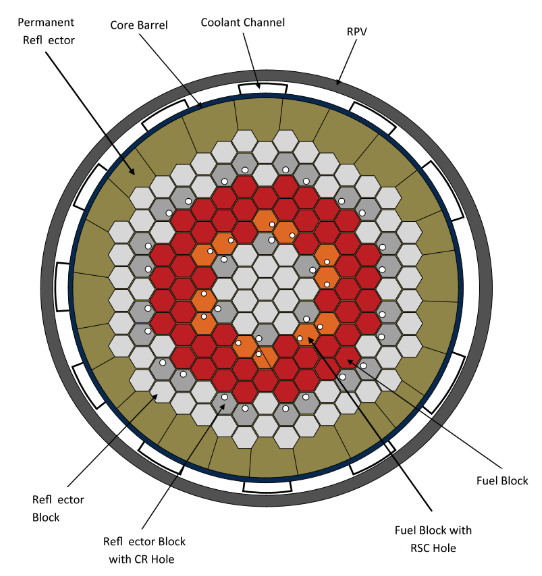
\includegraphics[width=\linewidth]{figures/radial-layout.png}
	% 		\caption{XY-plane.}
	% 	\end{subfigure}
	% 	\begin{subfigure}[t]{0.4\textwidth}
	% 		\centering
	% 		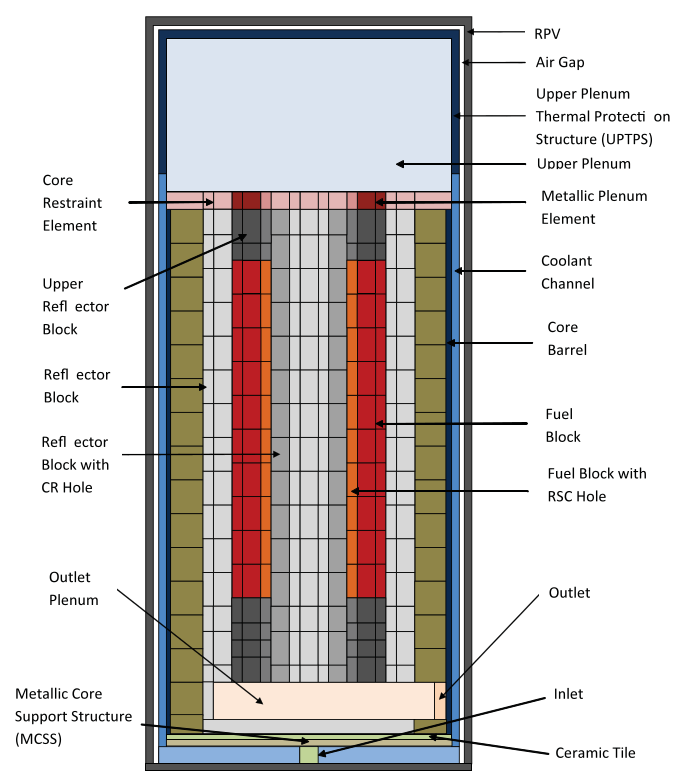
\includegraphics[width=\linewidth]{figures/axial-layout.png}
	% 		\caption{YZ-plane.}
	% 	\end{subfigure}
	% 	\hfill
	% 	\caption{MHTGR reactor layout.}
	% 	\label{fig:layout}
	% \end{figure}

	% \begin{figure}[htbp!]
	% 	\centering
	% 	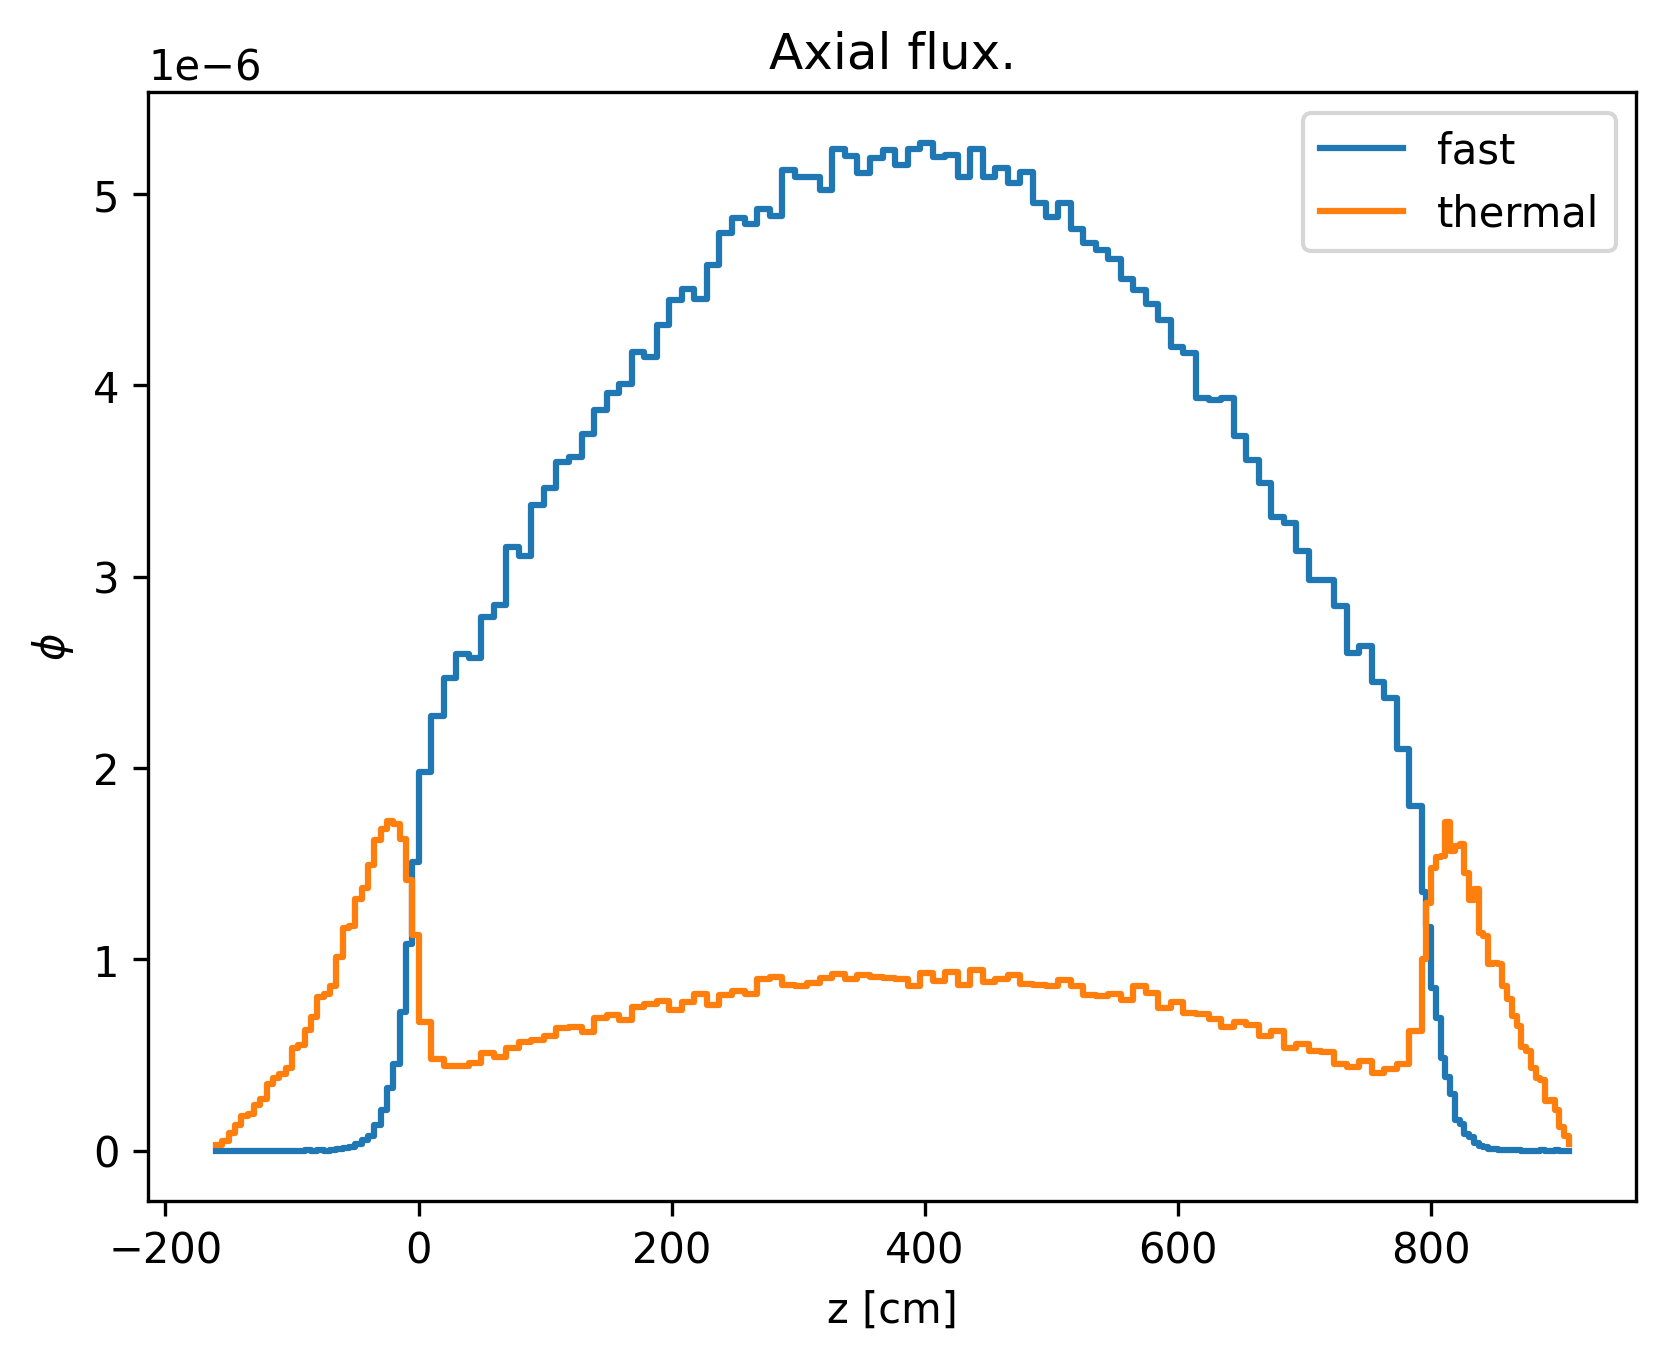
\includegraphics[width=0.6\linewidth]{figures/axial1.png}
	% 	\hfill
	% 	\caption{Neutron flux on the specified fuel channel.}
	% 	\label{fig:axial}
	% \end{figure}